\documentclass[12pt,letterpaper]{article}
\usepackage[top=0.85in,left=1in,footskip=0.75in,marginparwidth=2in]{geometry}

% use Unicode characters - try changing the option if you run into troubles with special characters (e.g. umlauts)
\usepackage[utf8]{inputenc}

% clean citations
\usepackage{cite}

% hyperref makes references clicky. use \url{www.example.com} or \href{www.example.com}{description} to add a clicky url
\usepackage{nameref,hyperref}

% line numbers
\usepackage[right]{lineno}

% improves typesetting in LaTeX
\usepackage{microtype}
\DisableLigatures[f]{encoding = *, family = * }

% text layout - change as needed
\raggedright
\setlength{\parindent}{0.5cm}
\textwidth 6.5in 
\textheight 9in
\renewcommand{\baselinestretch}{1.5}

% use adjustwidth environment to exceed text width (see examples in text)
\usepackage{changepage}

% adjust caption style
\usepackage[aboveskip=1pt,labelfont=bf,labelsep=period,singlelinecheck=off]{caption}

% remove brackets from references
\makeatletter
\renewcommand{\@biblabel}[1]{\quad#1.}
\makeatother

% headrule, footrule and page numbers
\usepackage{lastpage,fancyhdr,graphicx}
\usepackage{epstopdf}
\pagestyle{myheadings}
\pagestyle{fancy}
\fancyhf{}
\rfoot{\thepage/\pageref{LastPage}}
\renewcommand{\footrule}{\hrule height 2pt \vspace{2mm}}
\fancyheadoffset[L]{2.25in}
\fancyfootoffset[L]{2.25in}

% use \textcolor{color}{text} for colored text (e.g. highlight to-do areas)
\usepackage{color}

% define custom colors (this one is for figure captions)
\definecolor{Gray}{gray}{.25}

% this is required to include graphics
\usepackage{graphicx}
\graphicspath{{../figures/}}

% use if you want to put caption to the side of the figure - see example in text
\usepackage{sidecap}

% use for have text wrap around figures
\usepackage{wrapfig}
\usepackage[pscoord]{eso-pic}
\usepackage[fulladjust]{marginnote}
\reversemarginpar

% document begins here
\begin{document}
In this document, I have compared different essential gene predictors. These include BioTraDIS \cite{barquist_tradis_2016} (blue), log fold changes from Monte Carlo method \cite{turner_essential_2015} (green), P-values from running DESeq and Monte Carlo sampling (red), the ratio between the length of the longest uninterruped segment of the gene and the length of the gene (orange), and the average distance between insertion sites. The last two methods are selected from \cite{freed_combining_2016} Figure S3. To calculate one tailed P-values from two tailed P-values obtained from DESeq, I have divided the P-values by two, and if their corresponding logFC value was less than zero, pval = 1 - pval. The set of essential genes are obtained by comparing the genes in each strain to the essential genes in E.coli K-12 from ecogene study \cite{zhou_ecogene_2013}. The results are shown in Figure~\ref{fig:roc}
\begin{figure*}
\centering
\begin{tabular}{c c}
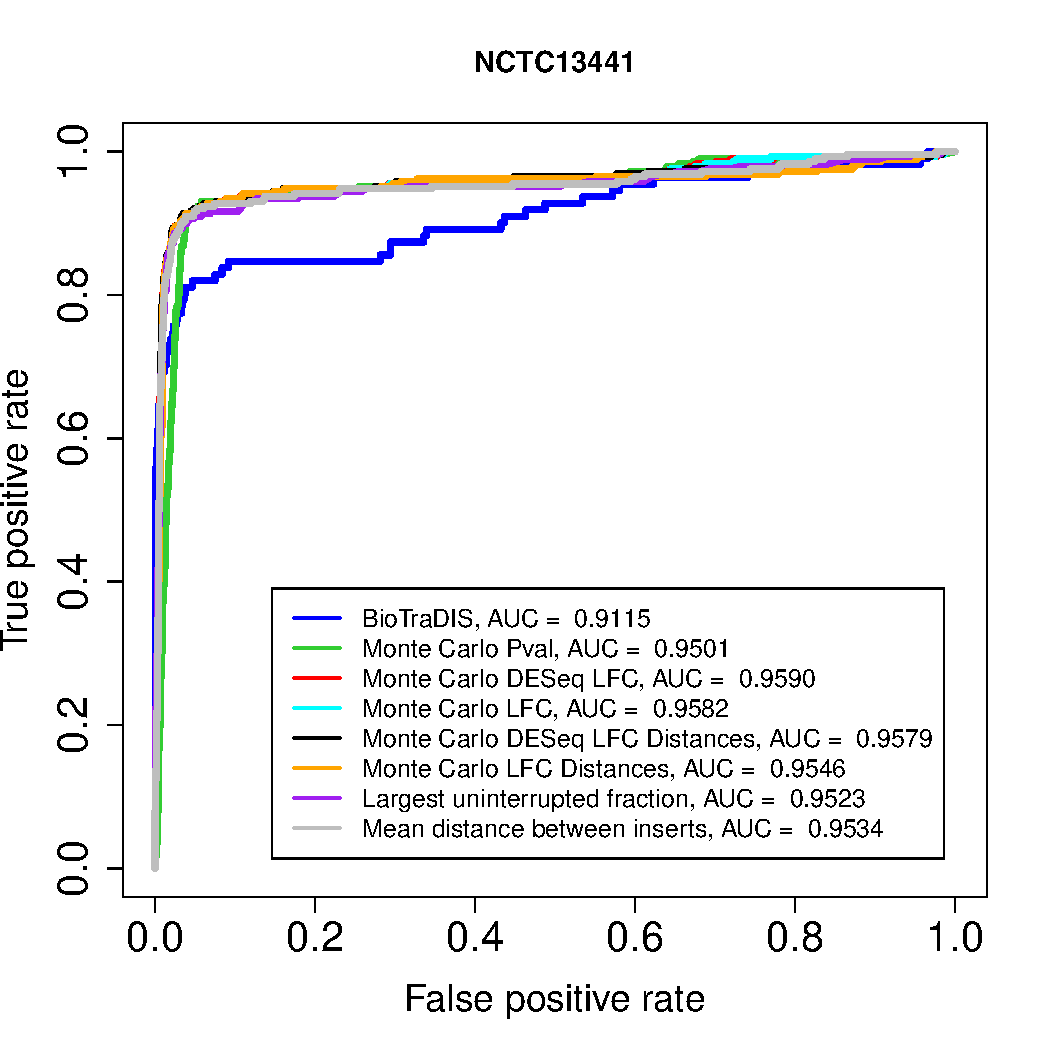
\includegraphics[page=1, scale=0.5]{essential-call-comparison-NCTC13441.pdf} &
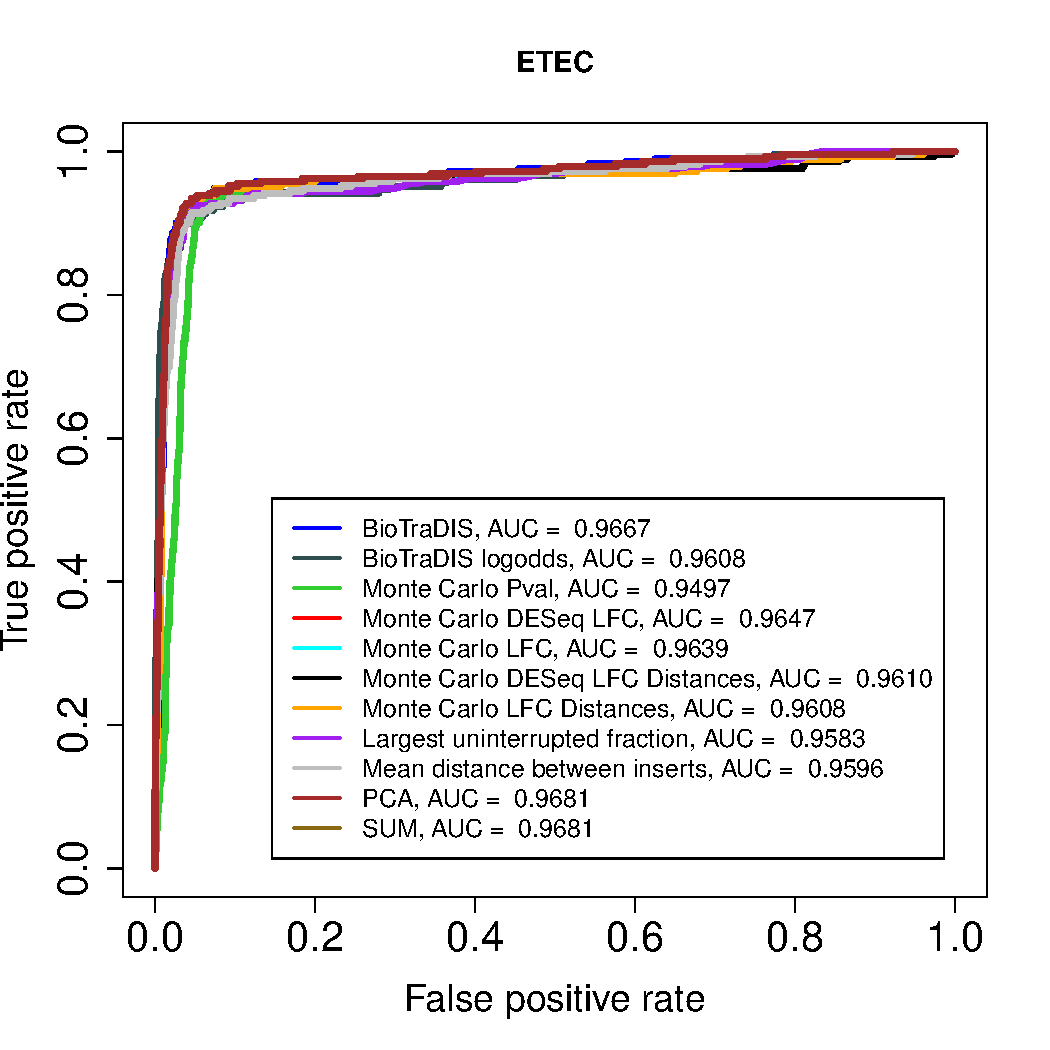
\includegraphics[page=1, scale=0.5]{essential-call-comparison-ETEC.pdf} \\
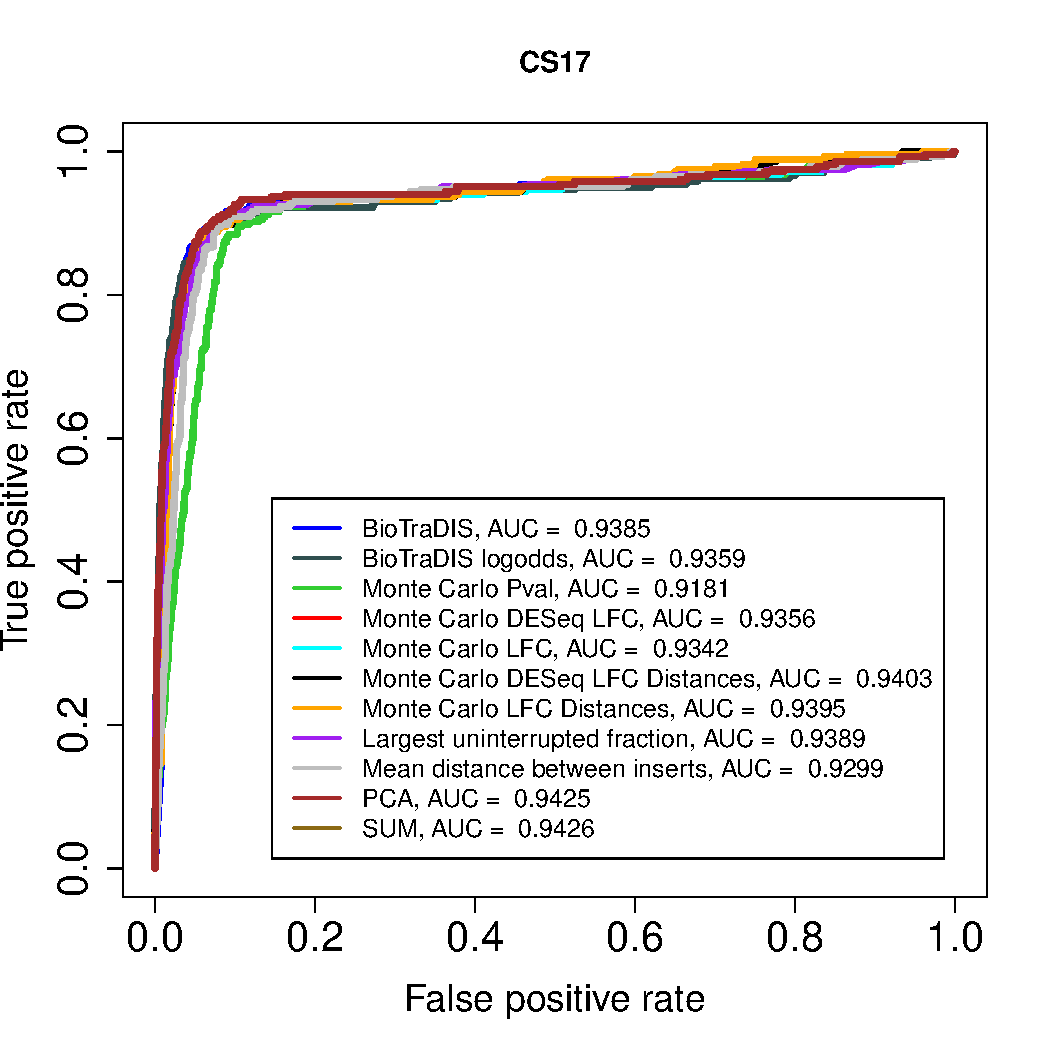
\includegraphics[page=1, scale=0.5]{essential-call-comparison-CS17.pdf} &\\
\end{tabular}
\caption{The comparison of different methods for calling essential genes in three E.coli strains.}
\label{fig:roc}
\end{figure*}

In Figure~\ref{fig:dotplot}, I have compared the logodds value obtained from BioTraDIS to both logFC and P-values from Monte Carlo method for CS17 strain.

\begin{figure*}
\centering
\begin{tabular}{c c}
\includegraphics[page=2, scale=0.5]{essential-call-comparison-CS17.pdf} &
\includegraphics[page=3, scale=0.5]{essential-call-comparison-CS17.pdf} \\
\end{tabular}
\caption{The figure shows the results of BioTraDIS vs. logFC from Monte Carlo method at left and BioTraDIS vs. DESeq P-values at right.}
\label{fig:dotplot}
\end{figure*}

In Figure~\ref{fig:hist}, I have plotted the distribution of each method. The essential and non-essential genes are well separated in Monte Carlo logFC, largest uninterrupted fraction, and mean distance between inserts. However, it is hard to distinguish between non-essential genes and beneficial losses in all these methods.

\begin{figure*}
\centering
\begin{tabular}{c c}
\includegraphics[page=4, scale=0.5]{essential-call-comparison-CS17.pdf} &
\includegraphics[page=5, scale=0.5]{essential-call-comparison-CS17.pdf} \\
\includegraphics[page=6, scale=0.5]{essential-call-comparison-CS17.pdf} &
\includegraphics[page=7, scale=0.5]{essential-call-comparison-CS17.pdf} \\
\end{tabular}
\caption{The figure shows the distribution of Monte Carlo logFC, Monte Carlo P-value, log2(largest uninterrupted fraction), and log2(mean distance between inserts)}
\label{fig:hist}
\end{figure*}

So far, Monte Carlo with logFC values is the best method. Interestingly, even though the mean distance between inserts and largest uninterrupted fraction methods are very simple, they work pretty well.

\bibliography{references}

%This defines the bibliographies style. Search online for a list of available styles.
\bibliographystyle{apalike}
\end{document}